\documentclass[conference]{IEEEtran}
\IEEEoverridecommandlockouts
% The preceding line is only needed to identify funding in the first footnote. If that is unneeded, please comment it out.
\usepackage{cite}
\usepackage{amsmath,amssymb,amsfonts}
\usepackage{algorithmic}
\usepackage{graphicx}
\usepackage{textcomp}
\usepackage{lipsum}
\usepackage{xcolor}
\usepackage{hyperref}
\def\BibTeX{{\rm B\kern-.05em{\sc i\kern-.025em b}\kern-.08em
    T\kern-.1667em\lower.7ex\hbox{E}\kern-.125emX}}
\begin{document}

\title{Synergy of Distributed Ledger Technologies and the Internet of Things*\\
% {\footnotesize \textsuperscript{*}Note: Sub-titles are not captured in Xplore and
% should not be used}
% \thanks{Identify applicable funding agency here. If none, delete this.}
}

\author{\IEEEauthorblockN{Sebastian Kanz}
\IEEEauthorblockA{\textit{Distributed Ledger Technologies} \\
\textit{MaibornWolff GmbH}\\
Frankfurt a.M., Germany \\
sebastian.kanz@maibornwolff.de}
% \and
% \IEEEauthorblockN{2\textsuperscript{nd} Given Name Surname}
% \IEEEauthorblockA{\textit{dept. name of organization (of Aff.)} \\
% \textit{name of organization (of Aff.)}\\
% City, Country \\
% email address or ORCID}
% \and
% \IEEEauthorblockN{3\textsuperscript{rd} Given Name Surname}
% \IEEEauthorblockA{\textit{dept. name of organization (of Aff.)} \\
% \textit{name of organization (of Aff.)}\\
% City, Country \\
% email address or ORCID}
}

\maketitle

\begin{abstract}
  The telecommunications company Cisco predicts that by 2030, more than 500 billion IOT devices connected to the Internet will have found their way into various areas of our daily lives \cite{cisco2016}. Networked objects of our everyday life such as refrigerators, coffee machines, the automated supply chain from the business environment or a smart city are only a few examples of this business field. Although the concept of IOT is still very theoretical, several use cases have already been developed. In order to fully exploit the great potential of IOT and to implement corresponding visions, a suitable IT solution must be provided for the corresponding use case. Many different manufacturers and service providers need a uniform platform on which they can network their IOT devices, services, business logic and customers with each other and integrate a secure payment system. The question arises whether and to what extent the two innovative technologies DLT and IOT can benefit from each other and whether DLT is suitable as a scaling, high-performance and secure technology for IOT use cases. To answer this question, this paper examines an exemplary IOT use case, creates a requirements analysis and determines a suitable DLT for validating the research question by means of a market analysis and a requirements assessment. Finally, the implementation of an exemplary prototype based on the selected DLT is used to validate the results of this thesis.
\end{abstract}

\begin{IEEEkeywords}
Blockchain, Distributed Ledger Technologies, Internet of Things, State Channel
\end{IEEEkeywords}



\section{Introduction}
\lipsum[1-1]


\section{Fundamental concepts}
\subsection{Distributed Ledger Technologies}
The terms Blockchain and Distributed Ledger Technology (DLT) are often used synonymously\footnote{In this paper the terms are also used synonymously, otherwise they are explicitly referred to.}, whereby Blockchain is a subclass of DLT \cite{mastering2017}. Basically, data in blockchains are combined into blocks and put in a fixed order using hash chains. DLT also uses structures other than blocks by arranging data, for example, through trees or graphs.\\

\begin{figure}[htbp]
\centerline{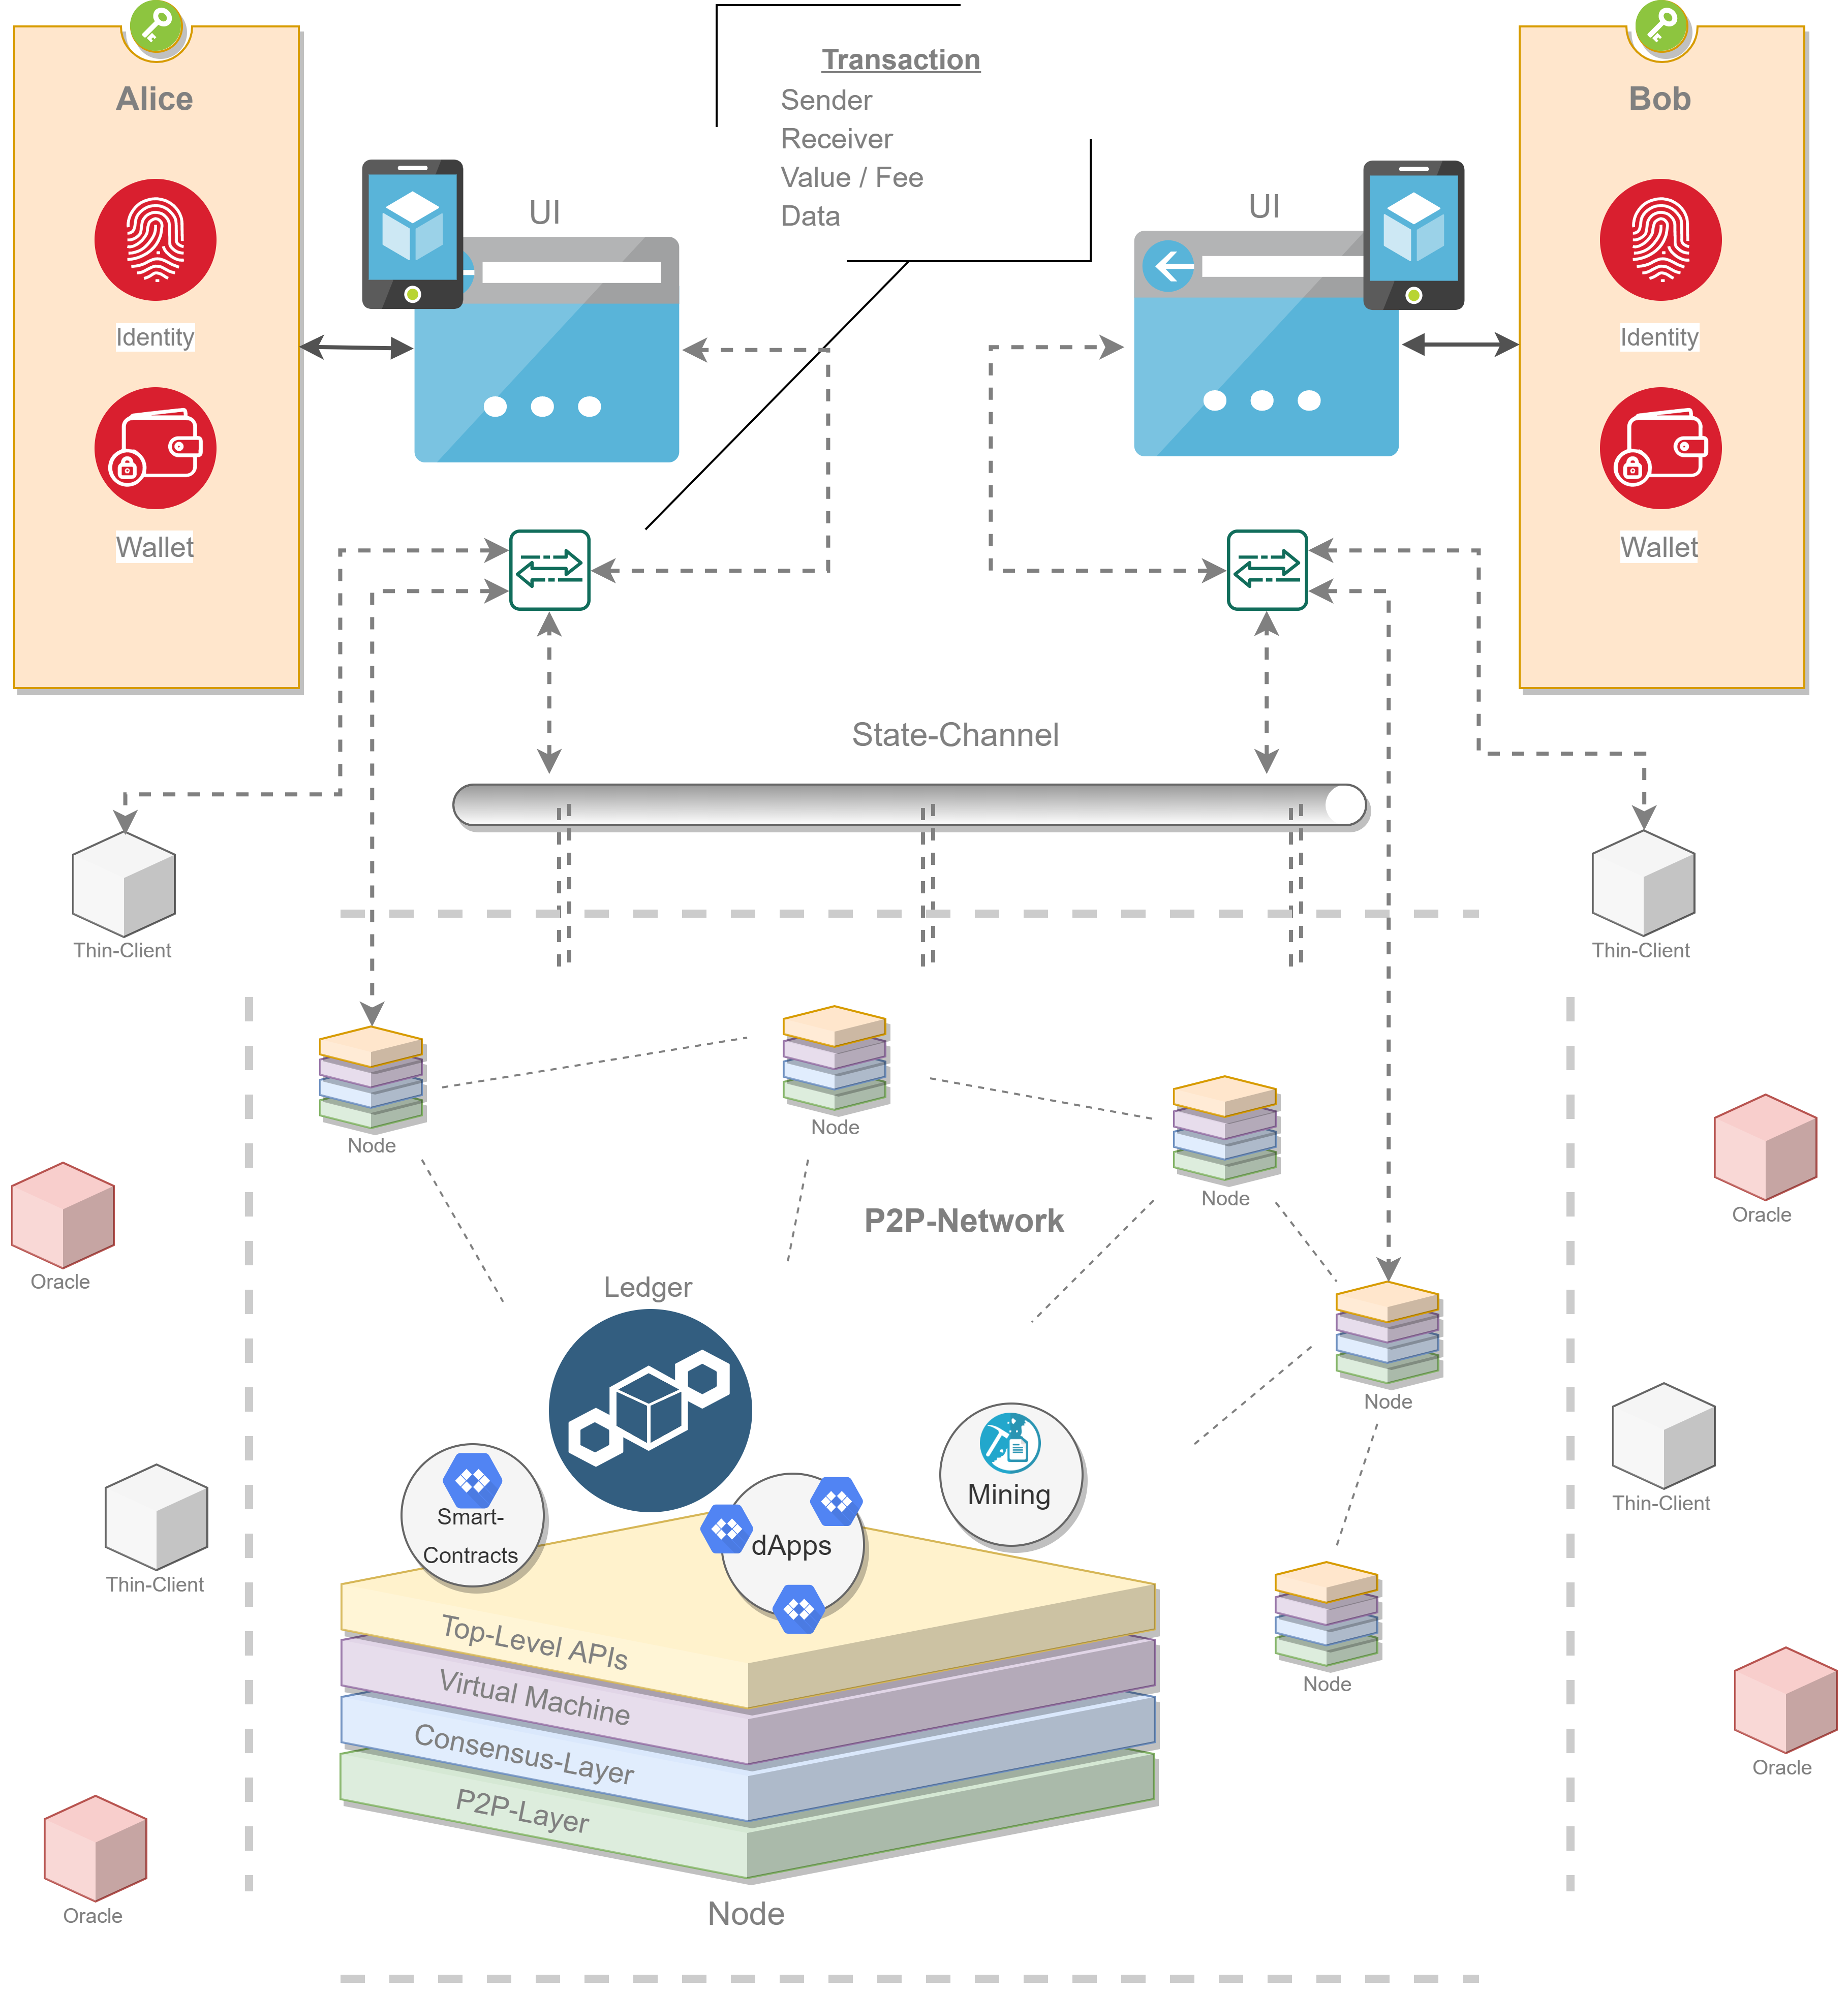
\includegraphics[width=0.5\textwidth]{Overview-DLT.png}}
\caption{Components of DLTs.}
\label{fig:overview-dlt}
\end{figure}

Figure \ref{fig:overview-dlt} shows the components of a DLT, whose interrelationships are described below and then explained in detail one by one.\\
DLTs are decentralized peer-to-peer (P2P) networks, in which nodes store data decentrally, use a consensus mechanism for synchronization and use asymmetrical encryption methods for system integrity and security. \cite{DLT2016}\\\
The main component of a Distributed Ledger is the ledger itself (German: Kassenbuch), which stores a history of all transactions made. A transaction represents a transfer of value or information between entity objects. It contains a sender, a receiver and a number of units to be sent. Depending on the implementation, additional content such as user data or software code can be added. This code, also called Smart Contract, is executed in a separate runtime environment (virtual machine). Through the interaction of several Smart Contracts one is able to execute entire applications onchain; this is called a distributed app (DApp).\\
Smart contracts can only access the internal (onchain) state of the ledger. If further (offchain) information is required\footnote{examples can be weather data, stock and exchange rates or lottery numbers}, these can be transmitted to the smart contract by so-called oracles. These act as 'trusted data providers', as the information provided cannot be validated. \cite{ORACLE2019}\\
Transactions executed by smart contracts, DApps or users must be validated by nodes on the network before they can be added to the ledger. To do this, they are combined by complex calculations (mining), added to the local ledger and then sent to other nodes.\\
The consensus log defines the rules for when a block may be added, which properties it must fulfill, and whether mining has been performed correctly. If any nodes are allowed to participate in the consensus, this is called a permissionless blockchain; if only privileged nodes are allowed to participate in the consensus, this is called a permissioned blockchain. Furthermore, blockchain networks can be classified as to whether transactions and blocks are publicly accessible and readable (public blockchain) or whether there are also restrictions (private blockchain).\\
Special requirements, such as the lowest possible transaction costs, a high transaction speed, a restricted scope of the application or restrictions due to the business model are some examples of admission restrictions and limited participation in the consensus procedure; depending on the given requirements, blockchain protocols must be selected or adapted for the respective application. All nodes that follow the consensus protocol and validate incoming blocks according to this protocol are called full nodes. There are also light clients (often thin clients), which only store parts of the ledger and usually only check the validity of the block headers. Just like oracles, light clients are not part of the P2P network, but access the nodes via an API.
If a user (represented in figure \ref{fig:overview-dlt} by Alice and Bob) wants to communicate with the blockchain or use it as a communication medium, this is also done via corresponding APIs. A graphical user interface allows users to initiate transactions, usually via browser or smartphone, and send them over the blockchain network. Each user has a wallet consisting of a public and a private key (Public / Private Key). The public key is similar to the account address of a bank account, the corresponding private key is similar to the PIN number. Thus, every user has a unique identity.\\
If Alice wants to send a transaction worth 10 € to Bob, she can do this in different ways. First, she can enter the desired information on her smartphone using a wallet app and send it to the Blockchain network at the touch of a button. This is received there via the corresponding API, processed and persisted in the ledger. Bob can also use his smartphone app to track when his account balance changes and who sent a transaction to his address.\\
An alternative solution to this would be the use of so-called state channels. These can be used by Alice and Bob to exchange any number of transactions with each other offchain and simply transfer the final balance of all exchanged transactions onchain to the ledger.\\


\subsection{Internet of Things}
The term Internet of Things - in short IOT - is a collective term and describes the networking of objects with each other (mostly via the Internet). It enables autonomous M2M communication, which in turn increases the degree of automation in the respective area of application. This means that communication between the IOT devices takes place autonomously, i.e. without human intervention. According to \cite{deloitte2018}, the subject area IOT can be divided into two areas Consumer IOT (CIOT) and Industrial IOT (IIOT). CIOT finds applications in the private environment, above all it is about smart home and the applications associated with it: Smart gardening, smart lights, intelligent door locking systems and heating controls. IIOT focuses on the commercial sector and tries to develop applications on a much larger scale: The automotive, energy and supply chain sectors are some of the important representatives here and appear as Smart Factory, Smart City, Connected Cars and others. The figure \ref{fig:overview-iot} gives an overview of the rough IOT architecture in the context of DLT.


\begin{figure}[htbp]
\centerline{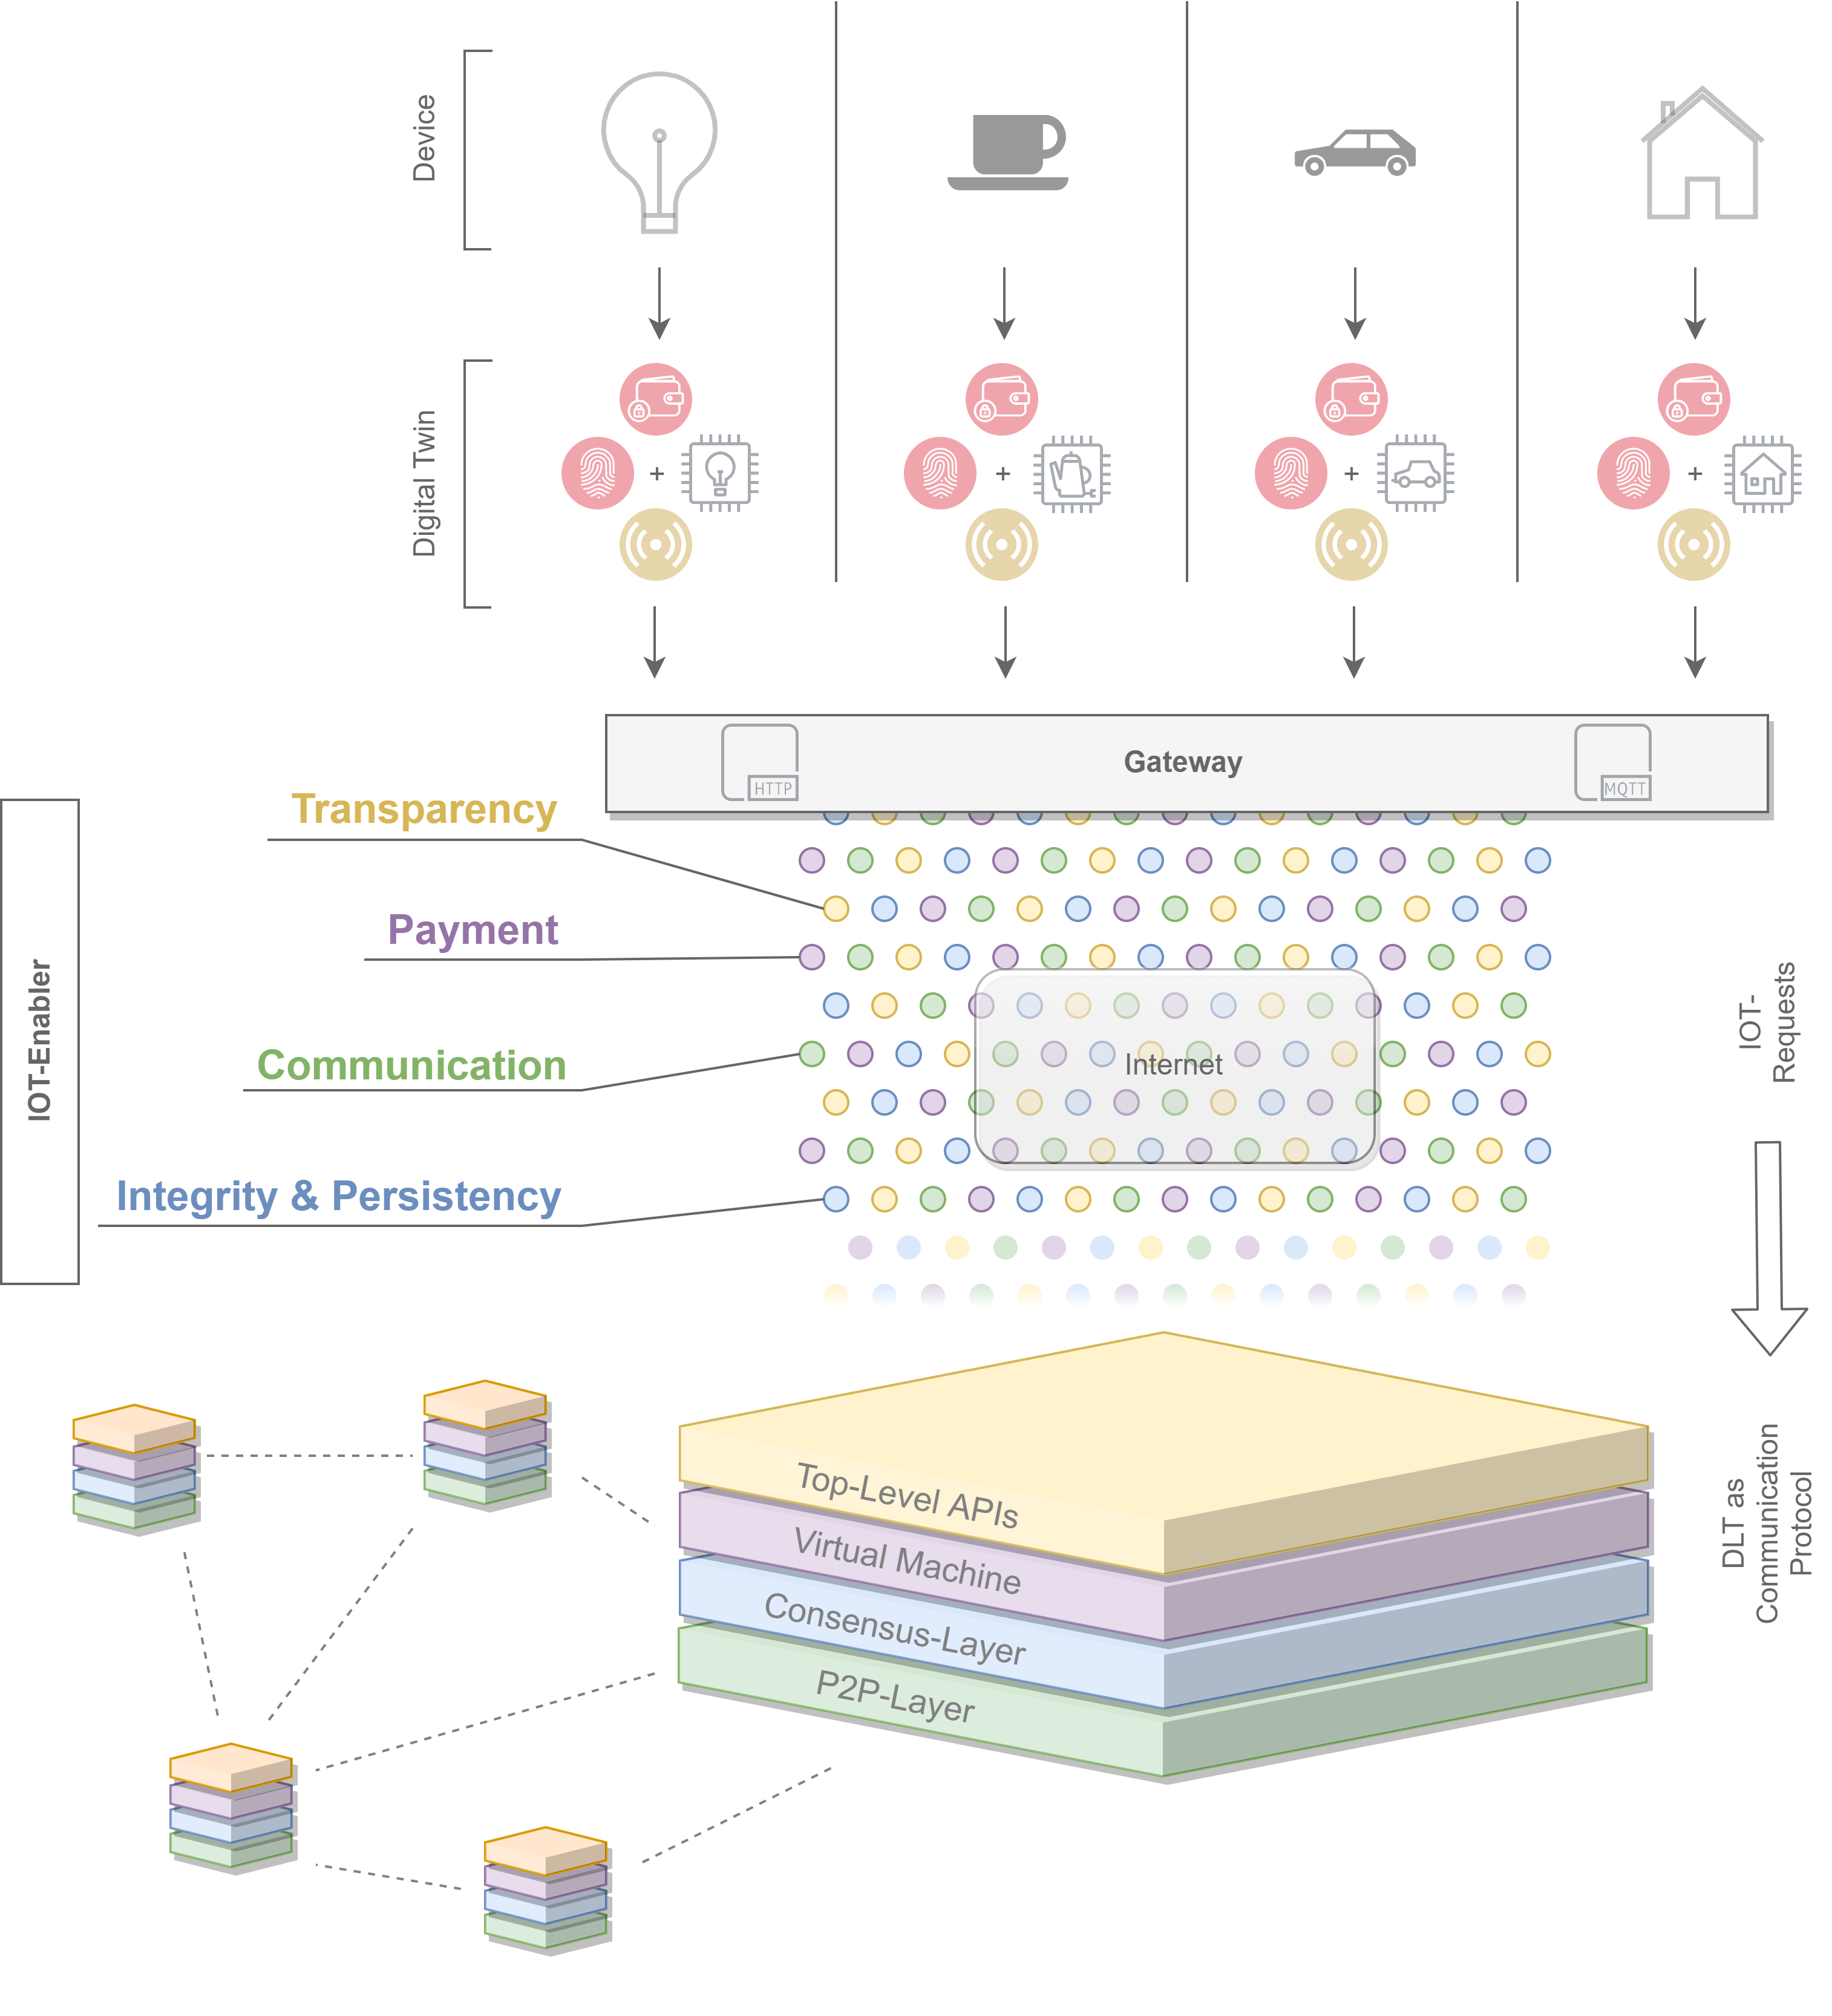
\includegraphics[width=0.5\textwidth]{Overview-IOT.png}}
\caption{Components of IOT.}
\label{fig:overview-iot}
\end{figure}


To network physical devices with each other, so-called digital twins are created. These are virtual images of the devices that are connected to each other by means of sensors and actuators. Thus, state changes can be transferred from the physical part to the virtual part and vice versa. Each device has a unique identity, which is mapped in the blockchain environment by means of decentralized identity (\textbf{Reference}). In addition, and depending on the application, devices have a wallet to perform automated payment processes M2M. Each device has a specific functionality and contributes to the IOT system. Devices are connected to the Internet via a local gateway, which may be a WLAN router or a mobile phone chip. Communication takes place via common communication protocols such as MQTT, HTTP or - as in the case of blockchain - via the blockchain protocol. IOT requests are processed via the blockchain network; the authors of \cite{SCIOT2016} formulate the benefits of this from the perspective of an IOT Device manufacturer and a consumer as follows:\\
\textit{´´From the manufacturer's side, the current centralized model has a high maintenance cost consider the distribution of software updates to millions of devices for years after they have been long discontinued. From the consumer's side, there is a justified lack of a trust in devices that phone home in the background and a need for a security through transparency approach.´´}\\
\cite{SCIOT2016} names two central core features of a Distributed Ledger: On the one hand, the distribution and the easy connection and accessibility of IOT devices, which can facilitate maintenance by the manufacturer. On the other hand, the authors address the question of trust on the part of customers with regard to data security and privacy. Here the blockchain technology according to \cite{SCIOT2016} ´´Security through transparency´´ and ensure greater acceptance.\\
However, the use of block chain technology is not always advisable or possible. For example, the use of a DLT in the IOT environment may be disadvantageous due to the use case or due to technical limitations and conditions. The first might be, for example, a smart home application that provides temperature control and monitoring of the home. A decentralized ledger would be oversized here and overqualified for this purpose. The cost would be disproportionate to the benefit. Furthermore, this IOT application case does not show any characteristics of a DLT application: It is a single party involved in a familiar environment with few terminals. On the other hand, technical hurdles can prevent the use of DLT. Especially in the automotive sector, the processing of sensor and actuator data in real-time is a critical point. Decentralized ledgers are not suitable for this purpose because they are not capable of running time-critical applications.\\
It becomes clear that the nature of the IOT application case makes a very decisive contribution to whether the use of a block chain solution makes sense or not. Due to its core features, the block chain offers some IOT enablers natively: Transparent and verifiable processes of all devices, integrated and automated M2M payment processing, P2P communication, and data integrity and persistence.

\subsection{State-Channels for asynchronous IOT use cases}
Blockchains\footnote{Note: This consideration is primarily concerned with public blockchains, regardless of the consensus method used. The scaling problem can usually be solved by limiting the blockchains to a private one.} have predefined limits due to their nature. A natural limit is given by the consensus protocol independent of block size and network capacity: For example, the Bitcoin network is limited to a block time of 10 minutes by the complex calculation of \textit{Proof-of-Work (PoW)}. If the block size is very small, blocks can be propagated over the network very quickly, but only a few transactions can be transmitted at once. If the block size is very large, it is very difficult for nodes to synchronize. Instead, more transactions can be transmitted at once.\\
Due to this limitation on block size and block duration, Bitcoin currently (as of 01/2020) allows an average of about 7 transactions per second \cite{Macdonald2017}. Other implementations may use different consensus mechanisms and other parameters, but there are natural barriers. It becomes clear that with increasing requirements, especially for transaction processing per time interval (mostly \textit{transaction per second (TPS)}, improved performance and new approaches to solutions become necessary. A solution is sought for the poor scaling of blockchains. \cite{Macdonald2017}\\
As a possible answer to the scaling problem of blockchains, so-called state channels are being developed. The goal is to process all kinds of status-changing operations off-chain, which are typically executed on the blockchain and stored on-chain. This reduces the number of accesses to the blockchain and the number of transactions, while at the same time improving the interaction time between individual parties. In the context of payments, this enables so-called micro-payments; state channels, which are limited to payment processing, are referred to as payment channels. These can be made faster and cheaper than normal transactions. The costs of such micro-payments can be kept very low because not all transactions are stored on the blockchain. \cite{Coleman2018}\\
The basic idea is the following: Alice and Bob reserve a portion of their assets on the blockchain so they can't dispose of them for the time being and open a payment channel to each other. This transaction, i.e. the opening of the payment channel, is stored on the blockchain. The volume of the channel, i.e. the assets that Alice and Bob can now exchange between each other, corresponds to the sum of the reserved assets. Your desired assets, which are to be reserved for the payment channel, can be reserved either by means of a multi-signature wallet (\textbf{Reference}) or smart contract (\textbf{Reference}). Alice and Bob now have a state of 50 Euro each. Afterwards both can send signed off-chain transactions to each other (i.e. not via the blockchain network). These transactions contain the new state: If Bob transfers 10 Euro to Alice, the state of Alice changes from 50 Euro to 60 Euro. If Bob sends another transaction of 10 Euro, the state of Alice changes to 70 Euro. Both of them can repeat this process as long as they want, as long as they are within the volume of 100 Euro. To close a channel, Alice or Bob send a transaction to the blockchain network containing the final state (in the example, Alice has 70 Euros and Bob 30 Euros). For a theoretically infinite number of transactions between Alice and Bob, only the opening and closing transaction of the payment channel must be stored onchain.\\
%https://busy.org/@bit-news/scalability-solutions-part-1
Another major advantage is the asynchronous nature of the transactions made possible by the state channel. If participants are not in the blockchain network (for example, due to connectivity problems), no transactions can be carried out. If real actions, such as opening a barrier or processing an action, are related to a blockchain status update, the real process would come to a standstill until the connection is restored if connectivity is lost. State channels could be used here to create a redundant connection that could also be used when the blockchain is not accessible. Some example implementations of state channels are Bitcoin's Lightning Network \cite{Lightning2016}, Ethereum's Raiden Network, or the implementation of Neo called Trinity \cite{Trinity2018}.\\
Another way to scale blockchain applications can be created by using side chains \cite{sidechain2019}. These are separate blockchains that run parallel to the main blockchain (also often called parent blockchain or main chain). To open a side chain, you must first prove that all assets whose status is to be changed in the side chain are locked or reserved on the main chain so that the owner cannot temporarily dispose of them (for example, through zero knowledge proofs, see \cite{zeroknowledge2020}). These locked assets can then be transferred to the side chain. There the status can be changed; for example, a money transaction can be executed. If an asset is to be transferred back to the main chain, proof must be provided that the asset has been locked on the side chain. This prevents effects such as double spending.\\
Solutions such as state channels and side chains are known as layer 2 approaches: This term refers to approaches that are not directly executed on the blockchain itself (layer 1), but on a separate system.\\
\textbf{Now what are the advantages in the context of IOT? Keywords: asynchronous processing, offline capability}


\section{Pay-As-You-Use renting of gastronomy devices}
\textbf{Description of use case goes here.}\\
\paragraph{Coffee Machines..}
\lipsum[1-1]

\subsection{Requirements}
\lipsum[1-1]

\subsection{Market analysis DLT}
\lipsum[1-1]

\section{Implementation}
\lipsum[1-1]


\section{Conclusion}
\lipsum[1-1]

\section{Future Work}
\lipsum[1-1]


% \begin{table}[htbp]
% \caption{Table Type Styles}
% \begin{center}
% \begin{tabular}{|c|c|c|c|}
% \hline
% \textbf{Table}&\multicolumn{3}{|c|}{\textbf{Table Column Head}} \\
% \cline{2-4}
% \textbf{Head} & \textbf{\textit{Table column subhead}}& \textbf{\textit{Subhead}}& \textbf{\textit{Subhead}} \\
% \hline
% copy& More table copy$^{\mathrm{a}}$& &  \\
% \hline
% \multicolumn{4}{l}{$^{\mathrm{a}}$Sample of a Table footnote.}
% \end{tabular}
% \label{tab1}
% \end{center}
% \end{table}

% \begin{figure}[htbp]
% \centerline{\includegraphics{fig1.png}}
% \caption{Example of a figure caption.}
% \label{fig}
% \end{figure}



\section*{Acknowledgment}
\textbf{Acknowledgment goes here}\\
\lipsum[1-1]



\bibliographystyle{IEEEtran}
\bibliography{IEEEfull,references}

\end{document}
